
%(BEGIN_QUESTION)
% Copyright 2006, Tony R. Kuphaldt, released under the Creative Commons Attribution License (v 1.0)
% This means you may do almost anything with this work of mine, so long as you give me proper credit

Automobile lifts used in repair shops are often powered by an ``oil under air'' pressure system.  Compressed air from the shop's compressor (used to power hand tools, pump up flat tires, clean parts, etc.) is readily available, and may be used as a source of pressure for a piston-and-cylinder lift machine.  Using compressed air means that there need not be a separate hydraulic pump to impart pressure to the oil used in the cylinder:

$$\includegraphics[width=15.5cm]{i00751x01.eps}$$

Which shut-off valve would be the safer one to close for halting the platform's upward motion when lifting an automobile off the ground?  Why? 

\vskip 10pt

If you were tasked with performing maintenance on this lift, how would you apply industry-standard ``lock-out, tag-out'' procedures to ensure a condition of {\it zero energy}?  Where would you apply locks and tags, and in what positions should these safety devices be placed in before the locks and tags are set?

\vskip 20pt \vbox{\hrule \hbox{\strut \vrule{} {\bf Suggestions for Socratic discussion} \vrule} \hrule}

\begin{itemize}
\item{} Piston seals leak, and can even fail catastrophically.  Describe the effect(s) of such a piston seal failure in this automotive lift, and also identify ways to make the system safe for the mechanic in the event of such a failure.
\item{} Identify where any additional valves may be placed in this system in order to more easily facilitate locking it out in a zero energy condition.
\item{} Is the size of the air/oil reservoir a factor in determining the lift's maximum weight capacity?  Why or why not?
\item{} Is the size of the ram's piston a factor in determining the lift's maximum weight capacity?  Why or why not?
\item{} Is the diameter of the air and/or oil piping a factor in determining the lift's maximum weight capacity?  Why or why not?
\item{} In a system where multiple devices need to be locked out for safety prior to maintenance, it is commonplace to use a {\it lock box} holding locks and keys for all these devices, then have maintenance people each place their own personal lock on the lid of this box so it cannot be opened.  Explain how such a ``lock-box'' system works to keep everyone safe.
\end{itemize}

\underbar{file i00751}
%(END_QUESTION)





%(BEGIN_ANSWER)

Shut-off valve \#1 (the oil valve) would be the safer one to close for halting the platform's vertical motion.

%(END_ANSWER)





%(BEGIN_NOTES)

Shut-off valve \#1 (the oil valve) would be the safer one to close for halting the platform's vertical motion.  With this valve closed, the platform will be hydraulically ``locked'' in place, unable to move either up or down with any external force applied to the platform.

\vskip 10pt

If shut-off valve \#2 were closed, and valve \#1 left open, the platform would stop rising, but it would still be able to move up and down with an external force.  If a mechanic were to tug on the platform, for instance, it would be able to move slightly if only valve \#2 were closed.

\vskip 10pt

The contrast between the consequences of one valve being shut versus the other is due to the {\it incompressibility} of oil and the {\it compressibility} of air.

\vskip 10pt

Incidentally, mechanical ``chocks'' are also used to secure a hoisted automobile in the air after lifting.  Mechanics wisely do not trust the cylinder to hold the automobile's weight, because pistons seals are known to leak, and sometimes fail catastrophically!










\vfil \eject

\noindent
{\bf Summary Quiz:}

Which shut-off valve would be the safer one to close in order to prevent the platform from moving after lifting an automobile off the ground?  Why?

$$\includegraphics[width=15.5cm]{i00751x01.eps}$$

\begin{itemize}
\item{} Valve \#2, because the compressibility of air ``locks'' the car in place
\vskip 5pt 
\item{} Valve \#1, because the incompressibility of oil ``locks'' the car in place
\vskip 5pt 
\item{} Valve \#1, because this prevents piston leakage from letting the car down 
\vskip 5pt 
\item{} Valve \#2, because this prevents leakage in the air/oil reservoir from letting the car down 
\vskip 5pt 
\item{} Valve \#1, because shutting valve \#2 would overload the air compressor
\vskip 5pt 
\item{} Valve \#2, because this helps prevent contamination of the oil by water in the air 
\end{itemize}


%INDEX% Mechanics, fluid power systems: hydraulic/pneumatic car lift
%INDEX% Physics, static fluids: compressibility
%INDEX% Process: automobile hydraulic lift
%INDEX% Safety, lock-out / tag-out: proper procedure

%(END_NOTES)


